\begin{pa} \label{PA:1.8}
Consider the function $y = g(x) = -x^2+3x+2$.
\begin{figure}[h]
\begin{center}
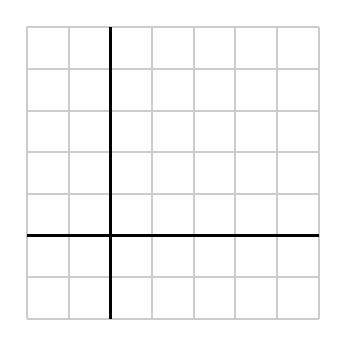
\includegraphics{figures/1_8_PA1.eps}
\caption{Axes for plotting $y = g(x)$ and its tangent line to the point $(2,g(2))$.} \label{F:1.8.PA1}
\end{center}
\end{figure}
\ba
	\item Use the limit definition of the derivative to compute a formula for $y = g'(x)$.
	\item Determine the slope of the tangent line to $y = g(x)$ at the value $x = 2$.
	\item Compute $g(2)$.
	\item Find an equation for the tangent line to $y = g(x)$ at the point $(2,g(2))$.  Write your result in point-slope form\footnote{Recall that a line with slope $m$ that passes through $(x_0,y_0)$ has equation $y - y_0 = m(x - x_0)$, and this is the \emph{point-slope form} of the equation.}.
	\item On the axes provided in Figure~\ref{F:1.8.PA1}, sketch an accurate, labeled graph of $y = g(x)$ along with its tangent line at the point $(2,g(2))$.
\ea
\end{pa} 

\afterpa

